\section{Zielsetzung}
\label{sec:Zielsetzung}
In diesem Versuch wollen wir die Funktionsweise einer Wärmepumpe, die Wärme von einem kälteren in ein wärmeres Reservoir transportiert, genauer betrachten.
Anschließend bestimmen wir die Güteziffer, den Massendurchsatz und die mechanische Kompressorleistung der Wärmepumpe, um diese qualitativ beurteilen zu können.  
\section{Theorie}
\label{sec:Theorie}
In diesem Versuch betrachten wir den Wärmetransport von einem kälteren in ein wärmeres Reservoir mithilfe einer Wärmepumpe.
Dafür benötigt man zusätzliche mechanische Arbeit.

\subsection{Arbeitsweise einer Wärmepumpe}
\begin{figure}
    \centering
    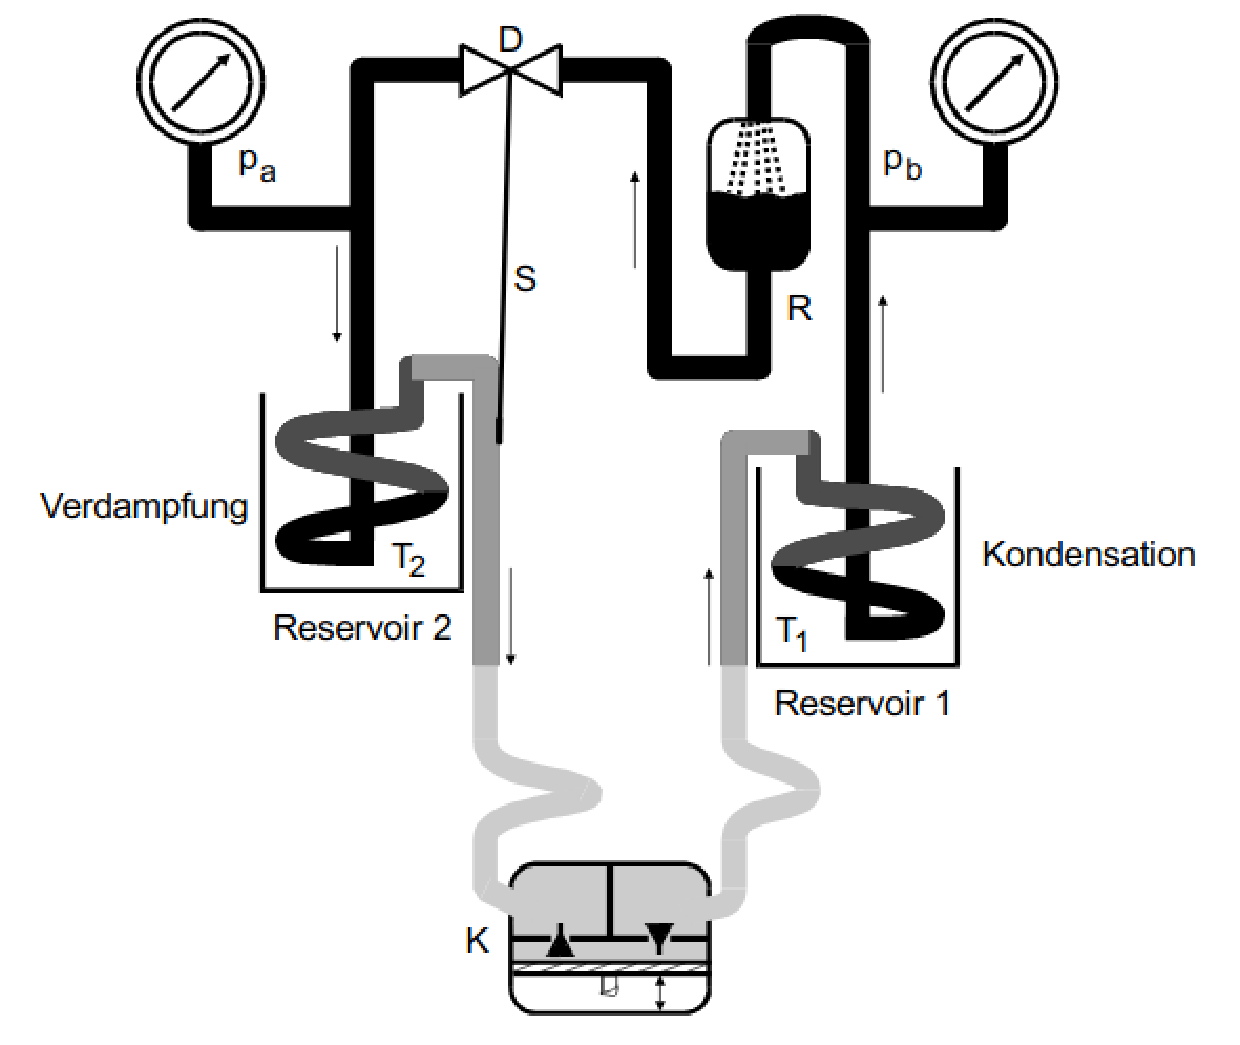
\includegraphics[width=\textwidth]{Aufbau_Waermepumpe.pdf}
    \caption{Prinzipielle Aufbau einer Wärmepumpe.\cite[3]{anleitung}}    
\end{figure}
Die Hauptbauteile einer Wärmepumpe sind ein Kompressor, zwei Reservoire mit Wasser und einem Drosselventil.
Das Transportmedium der Wärmepumpe sollte ein reales Gas mit hoher Kondensationswärme sein, da die Wärmeaufnahme  durch Verdampfen und die Wärmeabgabe beim Verflüssigen erfolgt.

Durch den Kompressor wird das Transportmedium durch das Reservoir 1, das Drosselventil D und das Reservoir 2 geführt.
Außerdem komprimiert er nahezu adiabatisch, also wird der Zustand des Mediums ohne großen Temperaturaustausch mit der Umgebung geändert.
In der Temperatur $T_2$ und  dem Druck $p_{\text{a}}$ soll das Transportmedium verdampfen und dabei die Verdampfungswärme L aufnehmen, 
bei der Temperatur $T_1$ und Druck $p_{\text{b}}$ kondensiert das Transportmedium und gibt L ab.
Das Drosselventil D lässt druckreguliert das Transportmedium durch, es befindet sich dort aufgrund des hohen Stromwiderstandes ein großer Druckunterschied.

Weitere Bauteile, wie der Reiniger R oder die Steuervorrichtung S, sorgen für einen störungsfreien Ablauf, sind aber für den eigentlichen Vorgang der Wärmeübertragung nicht notwendig.
Durch den Reiniger R werden Gasreste aus der Flüssigkeit entfernt, bevor diese durch das Drosselventil strömt.
Die Steuervorrichtung S reguliert das Drosselventil, sodass nur Gas in den Kompressor gelangt. 

\subsection{Die Güteziffer} \label{subsec:gueteziffer}
Die Güteziffer beschreibt das Verhältnis zwischen der übertragenen Wärme $Q_1$ und der dafür aufgebrachten Arbeit $A$.
Die übertragene Wärmemenge $Q_1$ setzt dich folgendermaßen aus $A$ und der dem kälteren Reservoir entnommene Wärmemenge $Q_2$ zusammen.
\begin{equation}
    Q_1 = Q_2 + A 
\end{equation}
Mit der Grundannahme, dass es keine Temperaturänderung der Reservoire gibt, folgt aus dem zweiten Hauptsatz der Thermodynamik im irreversiblen (realistischen) Fall:
\begin{equation}
    \frac{Q_1}{T_1 - \frac{Q_2}{T_2}} > 0
\end{equation}
, wobei $T_1$ und $T_2$ die Wassertemperaturen der Reservoire bezeichnet.
Daraus folgt für die Güteziffer in idealen Bedingungen:
\begin{equation}\label{eqn:idguete}
    \nu_{\text{id}} = \frac{Q_1}{A} = \frac{T_1}{T_1 - T_2}
\end{equation}
Dementsprechent ist der Arbeitsaufwand für die Pumpe geringer, je kleiner die Temperaturdifferenz $\Delta T = |T_1 - T_2|$ ist.

Da in der Auswertung die Temperaturkurven mit Funktionen angenähert werden, benutzen wir statt der Differenzenquotienten im folgenden Differentialquotienten.

Zur Berechnung der realen Güteziffer betrachtet man den gemessenen Temperaturunterschied von $T_1$ in bestimmten Zeitintervallen.
Mit der Wärmekapazität des Wassers aus Reservoir 1 $m_1c_w$ und der Wärmekapazität der Kupferschlange und der Eimer $m_kc_k$ gilt der Zusammenhang
\begin{equation}
    \frac{\symup{d}Q_1}{\symup{d}t} = (m_1c_w + m_kc_k) \frac{\symup{d}T_1}{\symup{d}t}.
\end{equation}
Für die Güteziffer ergibt sich dann 
\begin{equation}\label{eqn:gueteziffer}
    \nu = \frac{\symup{d}Q_1}{\symup{d}t \cdot N} = (m_1c_w + m_kc_k) \frac{\symup{d}T_1}{\symup{d}t} \cdot \frac{1}{N},
\end{equation}
wobei $N$ für die gemittelte Leistungsaufnahme des Kompressors steht.

\subsection{Der Massendurchsatz}
Ist die Verdampfungswärme pro Maase- und Zeiteinheit $L$ bekannt, lässt dich der Massendurchsatz über diese Formel berechnen:
\begin{equation}
    \frac{\symup{d}Q_2}{\symup{d}t} = L \cdot \frac{\symup{d}m}{\symup{d}t}
\end{equation}
Die pro Zeiteinheit aus dem Reservoir 2 entnommene Wärmemenge errechnet sich dabei aus der Temperaturänderung von $T_2$ .$m_2c_w$ entspricht der Wärmekapazität des Wassers in Reservoir 2.
\begin{equation}
    \frac{\symup{d}Q_2}{\symup{d}t} = (m_2c_w + m_kc_k) \frac{\symup{d}T_2}{\symup{d}t}
\end{equation}
Somit ergibt sich für den Massendurchsatz $\frac{\symup{d}m}{\symup{d}t}$:
\begin{equation}\label{eqn:massendurchsatz}
    \frac{\symup{d}m}{\symup{d}t} = (m_2c_w + m_kc_k) \frac{\symup{d}T_2}{\symup{d}t} \cdot \frac{1}{L}
\end{equation}

\subsection{Die mechanische Kompressorleistung}
Im allgemeinen gilt für die Arbeit $A_{\text{m}}$, die es braucht um das Gasvolumen $V_{\text{a}}$ auf das Gasvolumen $V_{\text{b}}$ zu verringern: 
\begin{equation*}
    A_m = - \int_{V_{\text{b}}}^{V_{\text{b}}} p\, \symup{d}V
\end{equation*}
Mit der Annahme, dass die Kompression adiabatisch abläuft, und der Poissonschen Gleichung, folgt für die Arbeit $A_{\text{m}}$ und somit auch für die mechanische Kompressionsleistung $N_{\text{mech}} = \frac{\symup{d}A_{\text{m}}}{\symup{d}t}$:
\begin{equation} \label{eqn:kompressorleistung}
    N_{\text{mech}} = \frac{\symup{d}A_{\text{m}}}{\symup{d}t} 
    = \frac{1}{\kappa - 1} \biggl( p_{\text{b}} \sqrt[\kappa]{\frac{p_{\text{a}}}{p_{\text{b}}}} - p_{\text{a}} \biggr) \frac{\symup{d}V_{\text{a}}}{\symup{d}t}
    = \frac{1}{\kappa -1} \biggl( p_{\text{b}} \sqrt[\kappa]{\frac{p_{\text{a}}}{p_{\text{b}}}} - p_{\text{a}} \biggr) \frac{1}{\rho} \frac{\symup{d}m}{\symup{d}t}
\end{equation}
In der Formel steht $\rho$ für die Dichte des Transportmediums im gasförmigen Zustand und $\kappa$ für das Verhältnis der Molwärmen (aus der Poissonschen Gleichung).
Man kann $\rho$ näherungsweise aus der idealen Gasgleichung errechnen.